\documentclass{article}

\usepackage{graphicx}

\begin{document}
\title{FYS-4150 Project 2}
\author{Yevhenii Volkov}
\maketitle

Link to github repository \\
https://github.com/YVol322/Comp-Phys/tree/Project-2/Project2

\section{Problem}
Show that $ \gamma \frac{d^2 u(x)}{dx^2}  =-Fu(x) $ can be written as $ A \vec v = \lambda \vec v $.\\
\\
$ \hat x \equiv \frac{x}{L} \Rightarrow x =\hat x L$;\\
\\
$\frac{d^2 u(\hat x)}{d \hat x^2} = \frac{d^2 u(\hat x)}{d(\hat x^2 L^2)} = \frac{1}{L^2}\frac{d^2 u(\hat x)}{d\hat x^2};$ \\
\\$\frac{\gamma}{L^2}\frac{d^2 u(\hat x)}{d\hat x^2}=-Fu(\hat x),\ \lambda \equiv \frac{FL^2}{\gamma};$\\
\\
$\frac{d^2 u(\hat x)}{d\hat x^2} =- \lambda u(\hat x). $\ Discretising this equation:\\
\\
$\frac{d^2u(\hat x_i)}{d \hat x^2} = \frac{u(\hat x_{i+1}) - 2u(\hat x_{i})+u(\hat x_{i-1})}{h^2} + O(h^2)$;\\
\\
$\frac{d^2v(\hat x_i)}{d \hat x^2} \approx \frac{v(\hat x_{i+1}) - 2v(\hat x_{i})+v(\hat x_{i-1})}{h^2}$.\\
\\
$i = 1: \frac{v(\hat x_{0}) - 2v(\hat x_{1})+v(\hat x_{2})}{h^2} = -\lambda v(\hat x_1);$\\
\\
$v(\hat x_{0}) = 0$;\\
\\
$ i= 1: \frac{2v(\hat x_{1})-v(\hat x_{2})}{h^2} = \lambda v(\hat x_1);$\\
\\
$ i= 2: \frac{-v(\hat x_{1}) + 2v(\hat x_{2})-v(\hat x_{3})}{h^2} = \lambda v(\hat x_2);$\\
\\
$...$\\
\\
$ i= n: \frac{-v(\hat x_{n-1}) + 2v(\hat x_{n}))}{h^2} = \lambda v(\hat x_n);$\\
\\
So we can write this equation in the matrix form $ A \vec v = \lambda \vec v $, where A is tridiagonal matrix of size $(n-1)\times(n-1)$ and $\vec v$ is an eigenvector, $\lambda$ is an eigenvalues.
\section{Problem}
C++ file to this problem pr2.cpp can be found om github repository.
\section{Problem}
C++ file to this problem pr3.cpp can be found on github repository.
\section{Problem}
C++ file to this problem pr4.cpp can be found on github repository.
\section{Problem}
Files to this problem can be found in github repository on folder pr5.
\subsection{Problem}
C++ file to this problem pr5.cpp can be found on github repo in folder pr5.\\
Data generated by this programme is saved to pr5table.csv.\\
Plot of this data and 2nd order polynomial fit pr5.png is generated by plotting script p5.py based on data from table pr5table.py.\\
From the plot pr5.png we can see that $N(j)$ is approximated by 2nd order polynomial with approximation coefficients: $[  1.69961807, 10.31209 , 14.86858518]$

\begin{figure}
  \caption{Tridiagonal A matrix.}
  \centering
    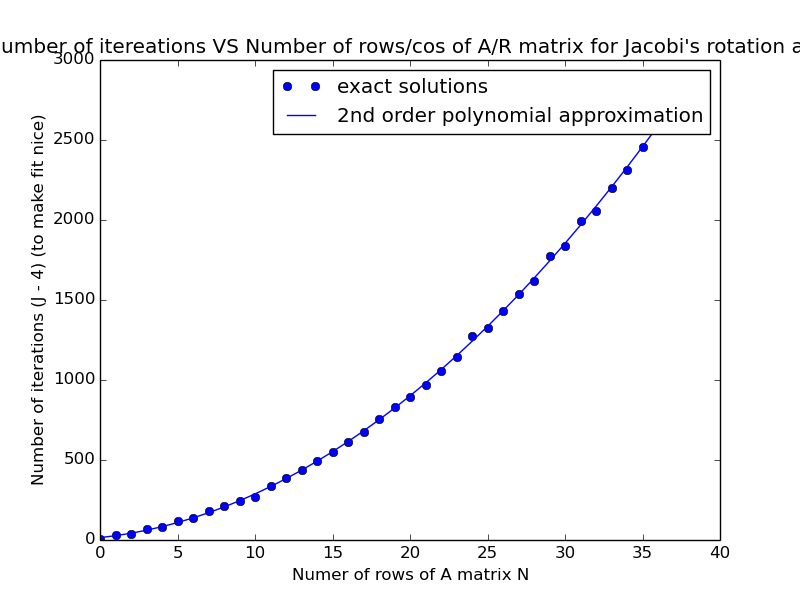
\includegraphics[scale=.5]{pr5.png}
\end{figure}

\subsection{Problem}
C++ file to this problem pr5.cpp can be found on github repo in folder pr5.\\
Data generated by this programme is saved to pr5btable.csv.\\
Plot of this data and 2nd order polynomial fit pr5b.png is generated by plotting script p5.py based on data from table pr5btable.py.\\
From the plot pr5b.png we can see that $N(j)$ is approximated by 2nd order polynomial with approximation coefficients: $[1.7016317, 8.49277389, 13.52447552]$\\
\\
We can see, that Jacobi's rotation method work approximately with the same amount of iterations for dense A matrix and for tridiagonal A matrix.\\
In my opinion, the reason is that this method does not really care how many zeros in matrix do we have. It cares only about largest off-diagonal elements, and this method transforming zeros in tridiagonal A matrix to non zeros.
\begin{figure}
  \caption{Dense A matrix}
  \centering
    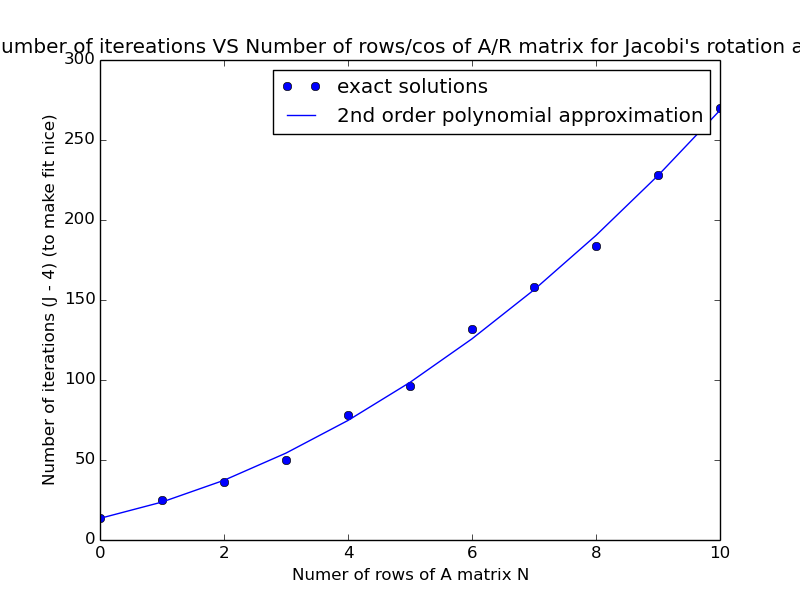
\includegraphics[scale=.5]{pr5b.png}
\end{figure}
\\
\\
\section{Problem}
Files to this problem can be found in github repository on folder pr6.
\subsection{Problem}
C++ file to this problem pr6.cpp can be found on github repo in folder pr6.\\
Data generated by this programme is saved to pr6table.csv.\\
Plots of this data pr6i.png is generated by plotting script p6.py based on data from table pr6table.py.
\subsection{Problem}
C++ file to this problem pr6b.cpp can be found on github repo in folder pr6.\\
Data generated by this programme is saved to pr6btable.csv.\\
Plots of this data pr6bi.png is generated by plotting script p6b.py based on data from table pr6btable.py.\\
\\
\\
\\
\\
\\
\\
\\
\\
\\
\begin{figure}
  \caption{Solution of dif. eq. for the lowest eigval (antisymetric), $n=10$.}
  \centering
    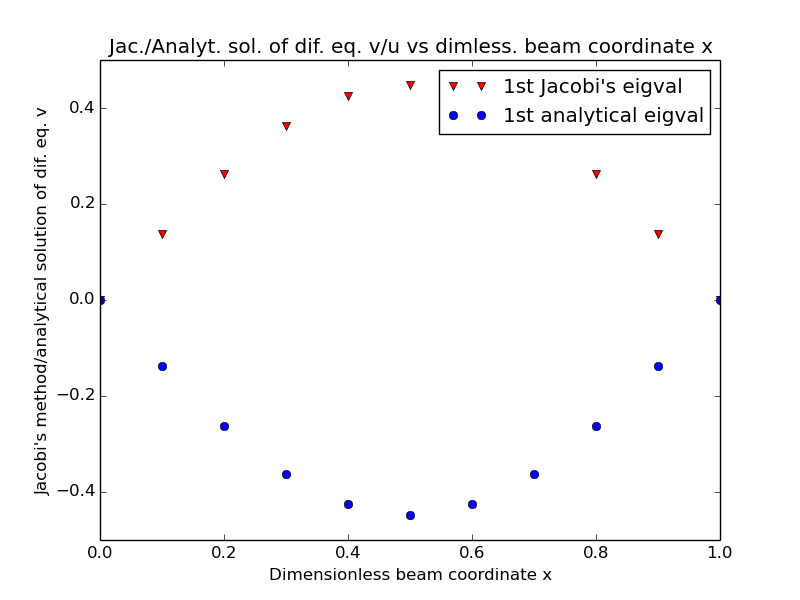
\includegraphics[scale=.5]{pr6a1.png}
\end{figure}
\begin{figure}
  \caption{Solution of dif. eq. for the lowest eigval (symmetric)), $n=10$.}
  \centering
    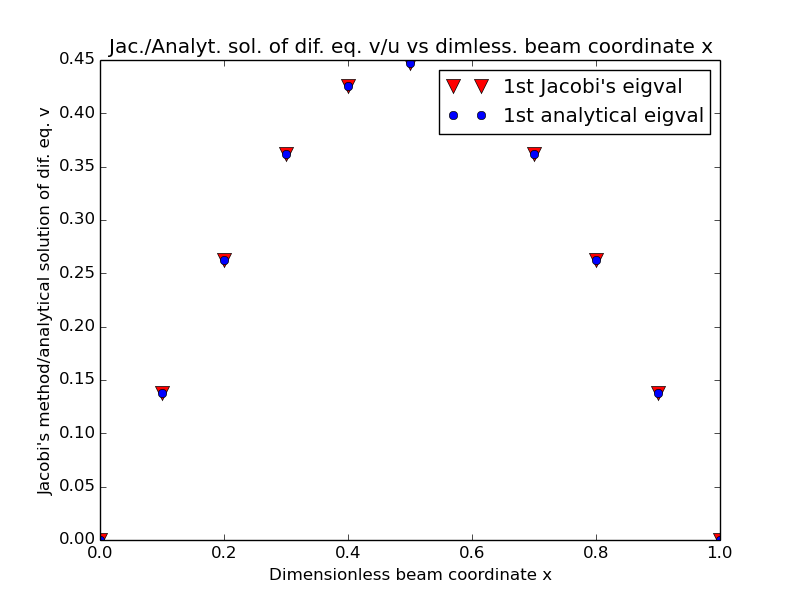
\includegraphics[scale=.5]{pr6a2.png}
\end{figure}
\begin{figure}
  \caption{Solution of dif. eq. for the 2nd lowest eigval (antisymmetric)), $n=10$.}
  \centering
    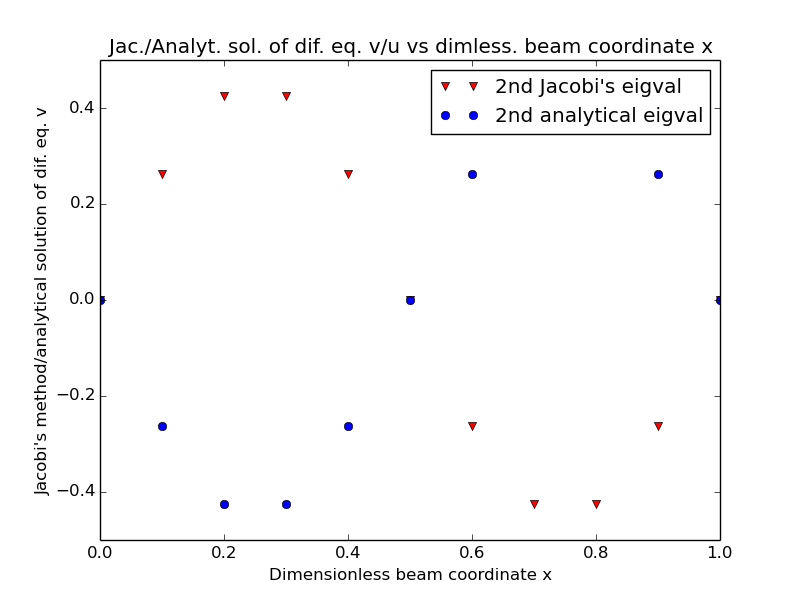
\includegraphics[scale=.5]{pr6a3.png}
\end{figure}
\begin{figure}
  \caption{Solution of dif. eq. for the 2nd lowest eigval (symmetric)), $n=10$.}
  \centering
    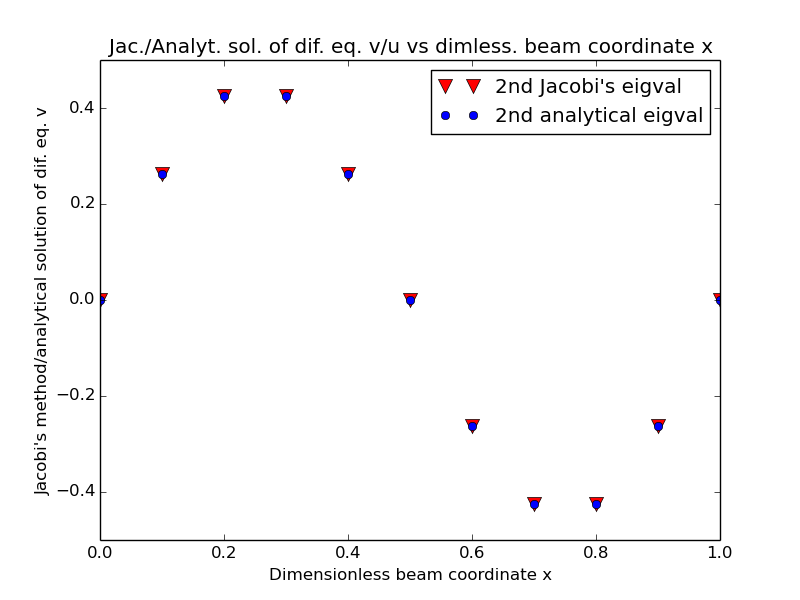
\includegraphics[scale=.5]{pr6a4.png}
\end{figure}
\begin{figure}
  \caption{Solution of dif. eq. for the 3rd lowest eigval (antisymmetric)), $n=10$.}
  \centering
    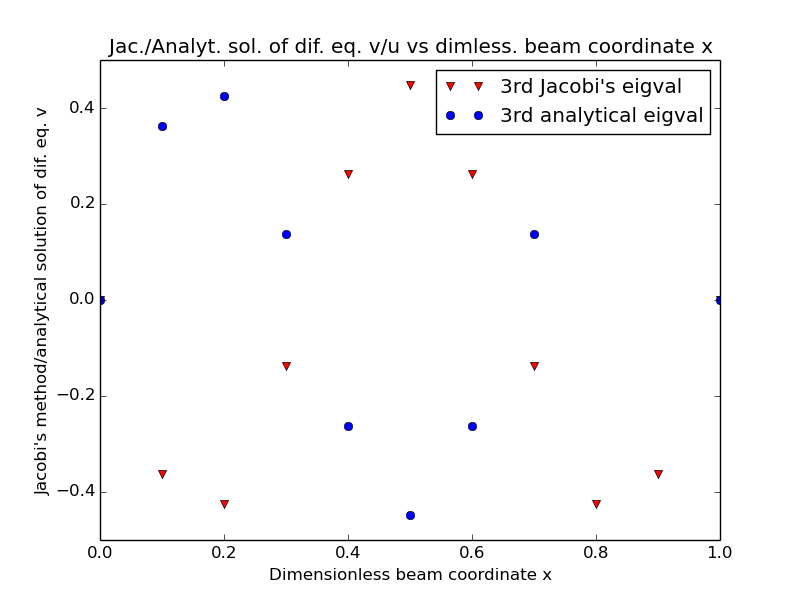
\includegraphics[scale=.5]{pr6a5.png}
\end{figure}
\begin{figure}
  \caption{Solution of dif. eq. for the 3rd lowest eigval (symmetric)), $n=10$.}
  \centering
    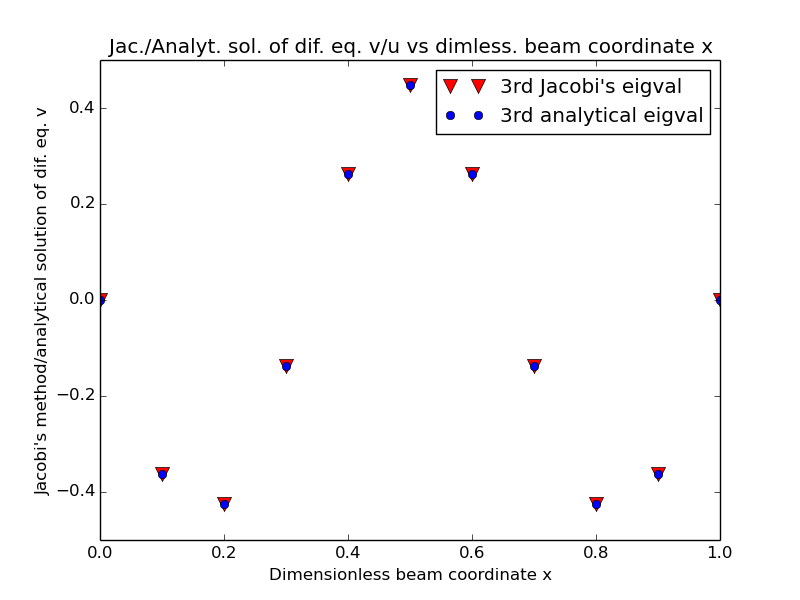
\includegraphics[scale=.5]{pr6a6.png}
\end{figure}
\begin{figure}
  \caption{Solution of dif. eq. for the lowest eigval (antisymmetric).), $n=100$}
  \centering
    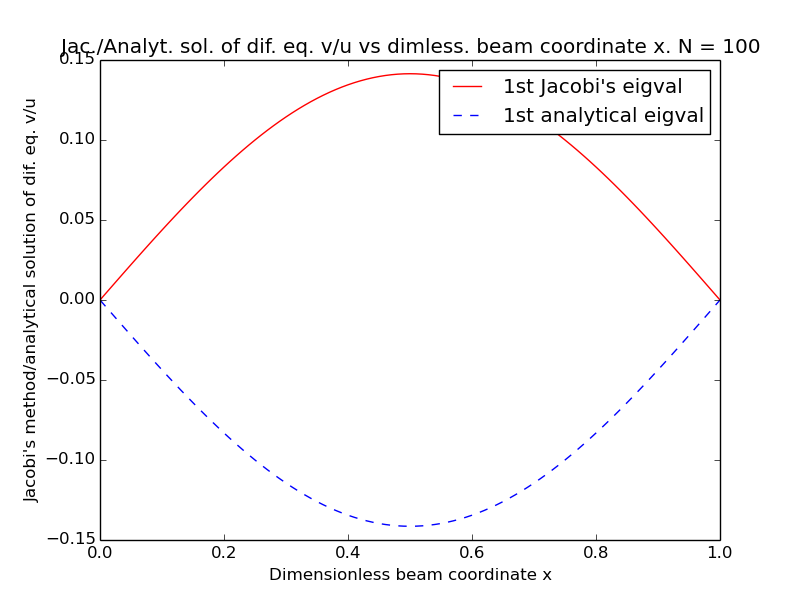
\includegraphics[scale=.5]{pr6b1.png}
\end{figure}
\begin{figure}
  \caption{Solution of dif. eq. for the lowest eigval (symmetric).), $n=100$}
  \centering
    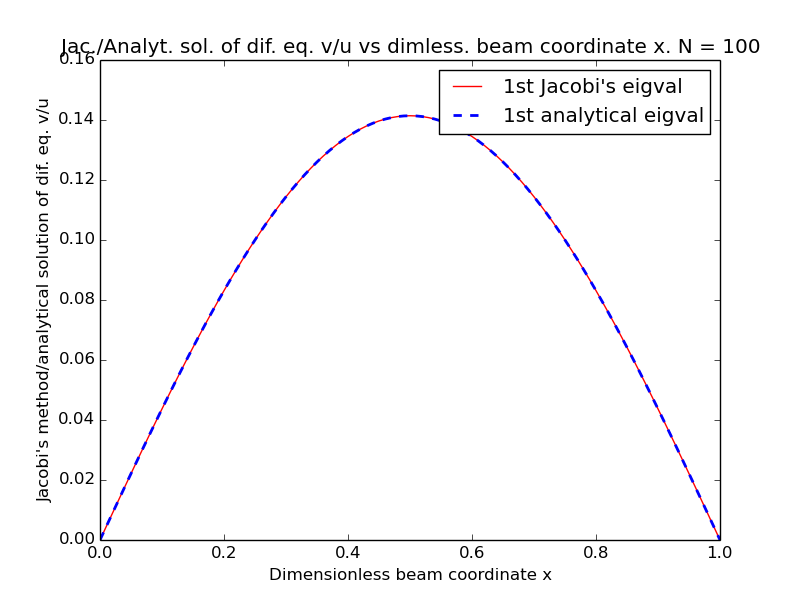
\includegraphics[scale=.5]{pr6b2.png}
\end{figure}
\begin{figure}
  \caption{Solution of dif. eq. for the 2nd lowest eigval (antisymmetric).), $n=100$}
  \centering
    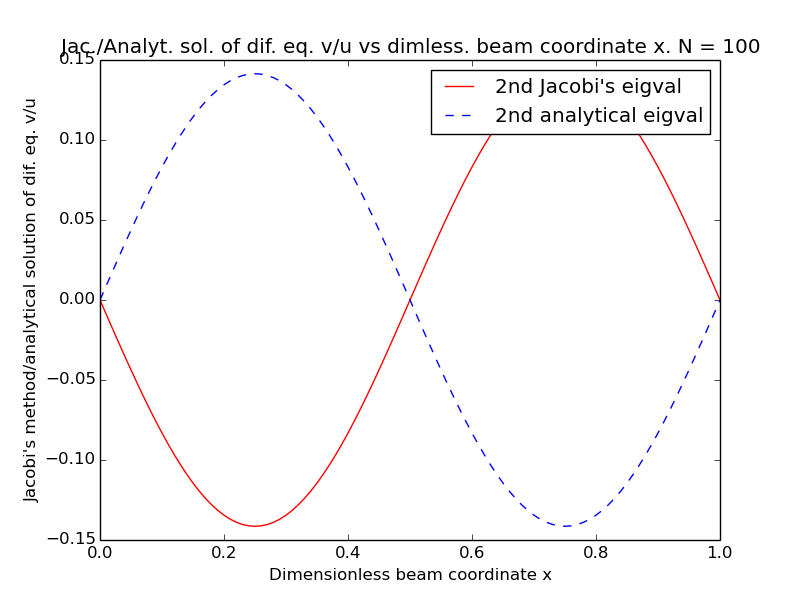
\includegraphics[scale=.5]{pr6b3.png}
\end{figure}
\begin{figure}
  \caption{Solution of dif. eq. for the 2nd lowest eigval (symmetric).), $n=100$}
  \centering
    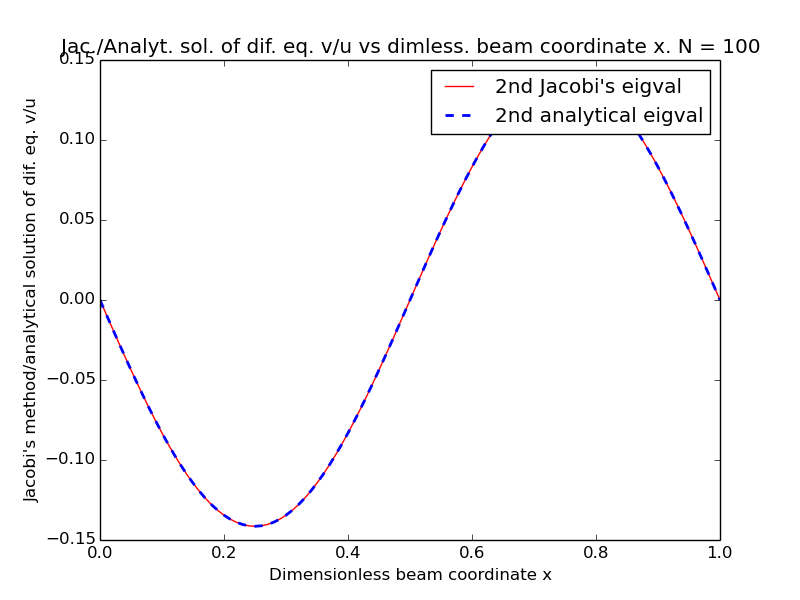
\includegraphics[scale=.5]{pr6b4.png}
\end{figure}
\begin{figure}
  \caption{Solution of dif. eq. for the 3rd lowest eigval (antisymmetric).), $n=10$}
  \centering
    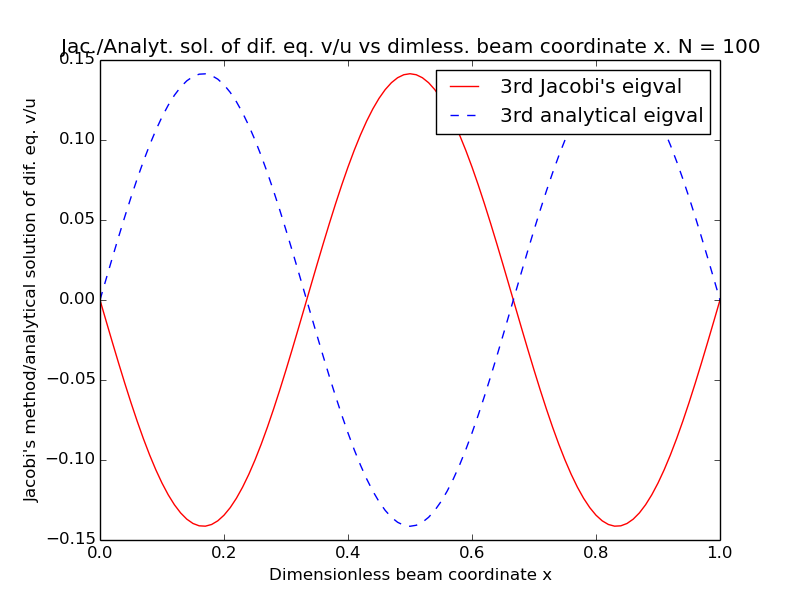
\includegraphics[scale=.5]{pr6b5.png}
\end{figure}
\begin{figure}
  \caption{Solution of dif. eq. for the 3rd lowest eigval (symmetric).), $n=10$}
  \centering
    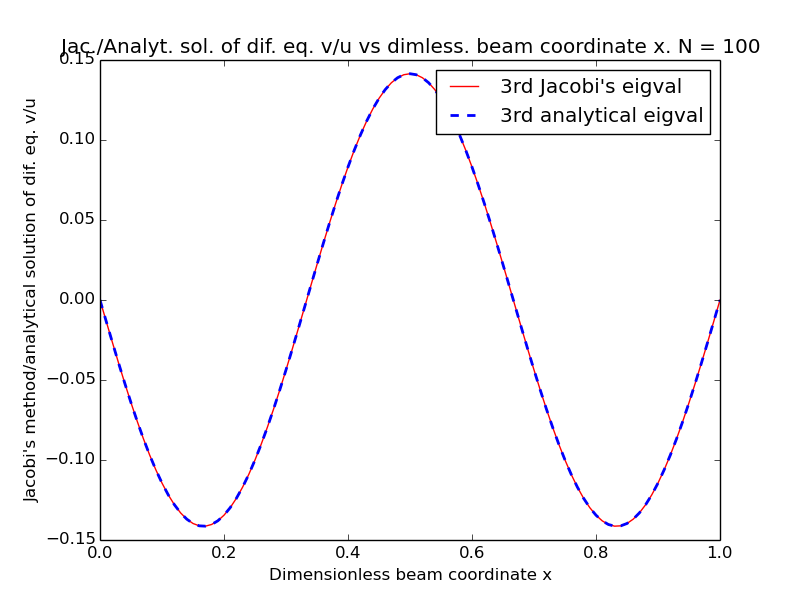
\includegraphics[scale=.5]{pr6b6.png}
\end{figure}



\end{document}